
\input{"header.tex"}
\input{"cover-referances.tex"}
\chapter{First Year report}

\label{c:First Year}

\section{Introduction}

%Nowadays, even if I close my door, and don’t talk to strangers about my private information, my privacy is still at risk because of the widespread of information technologies usage. Those new technologies can violate the community’s privacy, and therefore, there is no complete privacy anymore. By using social networks such as Facebook, Instagram, Twitter, MySpace, etc. we can discover a lot of details about others’ life, where he/she is now?, what he/she eats?, and who is with hem/her?, etc. Thus, revealing our private information could be used against our safety. Another critical matter is how our sensitive information such as name, address, phone number, credit card information, medical records, etc. maintained in the outside world, and what type of security regulations, safeguards, standards are in place to protect it? Recently, several major data breaches have accrued in both government and private organisations and caused massive financial and non-financial losses. A recent report ...............

\section{Literature Review:}
In this section, I have explored several relevant works and articles related to healthcare security, which is my research interest. The main objective is to get deeper insights of information technology trends, and their associated security challenges and opportunities in the healthcare industry. Specifically, how these technologies can harm or preserve patient information privacy.
\subsection{Health Information Technologies (HIS):}
% Introduction About HIS 

Healthcare industry is considered one of the most sophisticated businesses that interacts with a complex network of entities. Therefore, the use of information and communication technologies (ICT) in the healthcare sector has become imperative to support the activities of healthcare organisations. Hospitals often collect huge amounts of data to support their daily medical activities, as well as financial and managerial transactions, which have grown rapidly. Data at hospitals is generated from several sources, including patients, insurance companies, labs,pharmacy, etc. Thus, the management of such huge amounts of data requires an effective IT solutions that can satisfy many critical requirements such as easily accessible, cost-effective, reliable services and high quality.

% Definition and benefits of HIS

The need for technological advancements to improve healthcare services delivery, quality and performance have attracted the industry stakeholders to implement  several health information technologies. ISO 27799:2016 has defined Health Information Systems (HIS) as " \textit{a repository of information regarding the health of a subject of care in computer-processable form, stored and transmitted securely, and accessible by multiple authorised users}" \cite{TheInternationalOrganizationforStandardization2016}. Another definition of the HIS is based on the fact that it is a computer program, which  includes " a set of standards based on healthcare diagnosis, symptoms, cause, healthcare target and measurements" \cite{Pai2011}. The adoption of HIS have improved the compliance with the health care standards and disease control, which affect the overall quality delivery of healthcare services. Also, the implementation of clinical decision support tools have improved the diagnoses efficiency, which as a result have reduced significantly the total rate and time of healthcare utilisation. \cite{Care2006,Akowuah2013}.Currently, many healthcare organizations are utilizing the HIS as a backbone of their operational services because it ability to be integrated with hospital clinical care and administrative systems\cite{Rahim2016}.   

In this direction, several health information systems (HIS) have impacted positivity healthcare organisations such as E-Health, Electronic Mealth Records (EMR), Mobile health (mHealth),
and Telemedicine, cloud computing in healthcare, big data analysis, health exchange and health sensing \cite{WorldHealthOrganization2016,Yang2015}. 


\subsection{Electronic Medical Records (EMRs) systems:}

The  Electronic Medical Records(EMR) replaced paper-based charts in hospitals and medical clinics to an electronic version that may allow the patient information to be integrated, transmitted, stored and shared in different systems and locations \cite{Rahim2016}. It is difficult to find a stander definition for the EMR because the same meaning may refer to another term based on the perception of the EMR in a country or a healthcare sector.Thus,the EMR is considered a synonymous with abbreviations used elsewhere such as  Electronic Health Records(EHR)\cite{WorldHealthOrganization2016,Rahim2016,}, CPR (Computerized Patient Record),Protected Health Records (PHI) or Personal Health Records (PHR). In the other hand, several scholars have provided definitions that differentiated between those terms EMR, EHR and PHR \cite{Kierkegaard2011,Deutsch2010} . According to \cite{Yang2015,U.S.DepartmentofHealthandHumanServices2015}, three main differences of those terms  as the following:
\begin{itemize}
	\item\textbf{ Electronic Medical Record (EMR):} a health organisation is responsible to generate and control the EMR. Each EMR is a legal and digital record that includes all the patient medical history  during inpatient and outpatient visits. Basically, the EMR data are used for diagnoses purposes and shared locally within one health organization or institution\cite{Yang2015}. 
	\item \textbf{Electronic Health Record (EHR):} several health organisations are responsible to create,collect and maintain EHR data that are related to the patient healthcare.Thus, the EHR  may includes more comprehensive information as many sources contribute to it. Each EHR can be shared across different healthcare members , providers, regions, etc. When the EMR data are exchanged with external health organizations or entities, then they are considered EHR data and the EMR will be the main source of the transferred EHR\cite{Yang2015}.  
	\item \textbf{Personal Health Record (PHR)}: Each PHR record contains the same amount of EHR information, but the PHR data can be managed and accessed by individuals\cite{Yang2015,U.S.DepartmentofHealthandHumanServices2015}.
\end{itemize}

%\documentclass{article}
%\usepackage{graphicx}
%\graphicspath{ {images/} }

%\begin{document}
%	The universe is immense and it seems to be homogeneous, 
%in a large scale, everywhere we look at.
%\begin{figure}[h]
%\centering
%\includegraphics[scale=1]{Distunction_between_EMR_EHR_PHR}
%\caption{Differences between EHR, EMR and PHR (Adapted from )}
%\end{figure}
%\end{document}
The World Health Organization (WHO) \cite{WorldHealthOrganization2016} describes the Electronic Health Record systems (EHRs) as  " real-time, patient-centred records that provide immediate and secure information to authorized users. EHRs typically contain a patient’s medical history, diagnoses and treatment, medications, allergies, immunizations, as well as radiology images and laboratory results". Another report \cite{WorldHealthOrganization2013} stated that the implementation of the clinical decision tools, laboratory and pharmaceutical systems in poor African country such as Kenya, have reduced the practitioners errors and have enhanced both healthcare diagnoses and follow-up services. According to  \cite{OfHealth}, the implementation of EMR has provided healthcare organizations with significant advantages and can gain one or more of the following benefits:
\begin{itemize}
	\item \textbf{Better quality of care:} the EMR has improved the concept of information exchanging between doctors, healthcare team members and departments as well as off-site health providers. As a result, the patient information can be accessed easily if a patient needs an emergency care or requires a specific medication. Like any computer system, the system administrators can make a full backup of the EMR, which can decrease the risk and cost of losing data if a disaster accrued  \cite{OfHealth}.
	\item \textbf{Improved care efficiency:} the EMRs is receiving data from different health information systems, so the patient information can be modified from different sources and locations. This means that the patient data are available to several health practitioners, and each of them can communicate through the EMR. Thus, it can give doctors a simple way to review the patient medical history or request a specific test or task from others. Such communications way can reduce the side effects of repeating some medical procedures such as X-rays as well as the time and cost associated with it \cite{OfHealth}. 
	\item \textbf{Improved care convenient:} the patient history can be exchanged and accessed easily, which are the basic principles of the EMR. So, no need of physical carriage for the paper records or filling more paper forms, which in return can reduce the waiting time for both the patients and doctors to receive or review the medical records\cite{OfHealth}.
\end{itemize}

\subsection{Mobile Health (mHealth):}
%Write Why Privacy is a problem here, Put a justification
TBD

\subsection{Cloud computing in Healthcare}

Cloud computing is one of the newest IT paradigms, which emerged in 2007, and it allows customers to use many advanced IT services and resources through the internet at the cloud service providers’ data centre \cite{Sultan2014}. According to \citet{Buyya2009}, the importance of cloud computing will increase and soon be considered a fifth utility after water, gas, electricity, and telephone. Using a pay-per-use model, several organisations can improve their business’ services and IT function’s performance, efficiency and quality, by paying for what they are using of the IT resources and services \cite{Abdollahzadehgan2013}. Virtualization, utility computing, grid computing and internet services are the fundamental concepts of the cloud computing evolution. Thus, cloud technology is considered a solution that is applying new forms of IT outsourcing \cite{tashkandi2015cloud,Chang2013}.

There is not a universal definition or clear description for cloud computing, and according to some studies, there are more than 22 definitions for it \cite{Sultan2014}. The ISO/IEC 17788 defines cloud computing as "Paradigm for enabling network access to a scalable and elastic pool of shareable physical
or virtual resources with self-service provisioning and administration on-demand". According to \cite{BSI2014}, Cloud computing consists of seven services categories: Communications as a Service (CaaS), Software-as-a-Service (SaaS), Platform-as-a-Service (PaaS), Network as a Service (NaaS), Compute as a Service (CompaaS), Data Storage as a Service (DSaaS)and Infrastructure-as-a-Service (IaaS). These categories required several cloud deployment models to organise, control and share the physical and virtual resources such as the following: 
\begin{itemize} 
	\item \textbf{Public cloud}: it is a cloud deployment model, where the cloud service provider keeps the cloud services on premises and has full control on all physical and virtual resources related to the services\cite{BSI2014}. %The cloud services in a public cloud can be shared and accessed from several cloud service customers and can be owned and managed by an organisation, business, academia, etc. The availability and accessibility of cloud services for the cloud services customers are subjected to few restrictions\cite{BSI2014}.
	
	\item \textbf{Private cloud:} it is a cloud deployment model, where a single cloud service customer accesses the cloud services exclusively and has a control on all resources related to the services \cite{BSI2014}.%The cloud services in a private cloud can be shared and accessed based on cloud service customer authorization and can be owned and managed by a third party or the customer itself. In private cloud, the availability and accessibility of cloud services are limited and subjected to wide range of restrictions% \cite{BSI2014}. 
	
	\item \textbf{Community cloud}: it is a cloud deployment model, where a small number of cloud service customers access the cloud services exclusively, and at least one of customers can control resources, and it may exist on or off premises\cite{BSI2014}.% A community cloud can be owned, operated and managed by a third party or one or more customers in the cloud community. Unlike private cloud, the cloud service customers in the community cloud share the responsibilities and concerns of the service such as information security polices, procedures, requirements, etc\cite{BSI2014}. 
	
	\item \textbf{hybrid cloud:} it is a combination of two cloud deployment models, where appropriate technologies are in place to ensure the cloud services interoperability. A hybrid cloud may exist in or off premises and can be owned, operated and managed by a third party or an organisation itself\cite{BSI2014}.
	
\end{itemize}

In the healthcare industry, cloud computing has many promises. Due to the complexity of hospital information systems (HIS), cloud computing is a solution that opens a new horizon for patients’ records to be accessible via a secure authentication by authorised healthcare providers\cite{Grindle2013}.Also, it will help healthcare providers to gain important cost reductions and save money that is usually spent in buying and maintaining the needed hardware and software \cite{ahuja2012survey,Masrom2014}.

However, many organisations in different industries worldwide are still not ready to adopt cloud computing services. According to a recent report \cite{MarketsandMarkets}, the healthcare cloud computing market is predicted to grow nearly 9.48 billion dollars between 2015 to 2020, and only 4 percent of prospective cloud customers are healthcare organisations.The reasons for low adoption of cloud computing technology in healthcare industry are attributed to security and privacy fears, IT regulations compliance burdens, resource control and vendor lock-in concerns, as well as the lack of understanding of the technological, organisational and environmental factors that affect the decision makers when considering such technological shift \cite{MarketsandMarkets,tweel2012examining}.
\\
According to \citet{Mu2011}, the level of trust and effectiveness of the security and privacy controls is one of the management main challenges that hinder health cloud adoption. Thus, health cloud provider must show a strong commitment to protecting sensitive data of the health care customer. Uncertain compliance with cloud-related security regulations, best practices and policies may lead to increase privacy risks, which at the end raise resistance to adopt health cloud. Also, several countries have various regulation how the patient data should be stored, processed, and transferred.\cite{Mu2011} reported that the nature of cloud computing may include separate storage locations in different countries, which as a result may cause serious legal problems between the health cloud providers and their customers. This type conflict may evoke different privacy threats such data leakage or disclosure of patient data to unauthorized parties.

%Write Why Privacy is a problem here, Put a justification
% Add some studies here about Cloud computing in Healthcare


%\subsection{Internet of Thing (IoT) in Healthcare}

%Write Why Privacy is a problem here, Put a justification

\subsection{Information Security Managment(ISM) In Healthcare:}
Nowadays, Information and Communication Technologies (ICT) an important success factor within any modern society. Many new technologies have emerged and have improved people lives and organizations’ services including governments, worldwide. The significant shift in the business environment, economic instability, and customers’ desires and expectations, increase the need to develop and adopt new IT innovations. Over the last decades, several strategic transformations in enterprises and the governmental sectors are based on ICT applications, which brought a lot of benefits. Consequently,the need for Information Security (InfoSec) becomes an essential matter as thousands of organizations worldwide are heavily dependent on information process systems to perform their daily tasks. Thus, it is a critical role to ensure that the information technology assets are secured and protected against IT threats.
Many scholars have defined "information security" from different perspectives as it includes multidimensional factors that are concentrated on the preservation and protection of information assets via the implementation of security technical,operational and physical controls \cite{Hamid2014,Posthumus2004}. While those controls  need to be improved, reviewed and monitored in regular bases to ensure that the organizations' business and security objectives are achieved\cite{ISO/IEC2014}.


The national institute of Standard and Technology (NIST)\cite{Kissel2013} has defined information security as "the protection of information and information unauthorised access, use, disclosure, disruption, modification, or destruction in order to provide confidentiality, integrity, and availability ". \citet{Zafar2009}, they incorporate more components to InforSec definition in order gain a holistic view. These components are: establishing security policies and procedures, understanding and assessing potential security threats and risks, implementing and monitoring security controls, educating and training personnel in security awareness, performing permanent technology assessment and integrating information security governance. Information security mainly aims to preserve information confidentiality, unauthorised integrity and availability, which is known as (CIA) security triad\cite{pfleeger2007security}.Also \cite{ISO/IEC2014} adds authenticity, accountability, non-repudiation and reliability . According to European Network and information Security Agency (ENISA)\cite{ENISA2006},information confidentiality means "The protection of communications or stored data against interception and reading by unauthorized persons" . Integrity is refereed to "The confirmation that data which has been sent, received, or stored are complete and unchanged." Availability is defined as "The fact that data is accessible and services are operational". 


% Health information systems security standards
The sensitive nature of health information over other personal information and the growth rate of dependency on health care information systems, have increased the need to robust information Security Management (ISM). If patients' information has been compromised, then the health organisation may suffer from lots of legal issues, which may turn to financial losses as well as a huge damage to the organisation reputation. Furthermore,the HIS now have been shifted from stand-alone system with specific end-users to includes patients at homes via the internet. This development in network and information exchange technologies have increased the type and capacity of the HIS threats and challenges.Such development in network and information exchange technologies have increased the type and capacity of the HIS threats and challenges \cite{Hsu}. 
In response to these security risks, initiatives from several countries and institutions have been launched to improve ISM practices, procedures and guidelines by developing many generic and specific security standards. These standards aim to help the organisations in several industries to utilise their resources and efforts efficiently in order to gain an adequate security level via the adoption of best security practices \cite{Rahim2016,Akowuah2013}.


\citet{Akowuah2013} in their literature survey have reviewed several security standards including NIST Special Publication 800-53 , HITRUST Common Security Framework (CSF), Control OBjective for Information and related Technology (COBIT), ISO/IEC27002:2005, ISO/IEC27001:2005, ISO27799:2008, ISO17090:2008,ISO/TS 25237:2008. \cite{Akowuah2013} aim was to facilitate the choosing process for a suitable security standard that can guide information security management practices in the healthcare industry.In this survey, many standards were reviewed and analysed in order to assist IT management in their initial steps toward security programs implementation. \citet{Akowuah2013} suggested that ISO 27799:2008 and its associated series ISO 17090:2008 and ISO/TS 25237:2008 were more suitable of all size organizations in the healthcare industry as they were tailored to handle various security aspects and technical issues within healthcare environment. Moreover, Health Information Trust Allianc (HITRUST) is a specific health security standard that can satisfy many big size organizations security needs. It requires a subscription with HITRUST to get an access for health information security materials and training courses.In the other hand, some security standards such as NIST SP 800-53, ISO 27002:2005, and COBIT were more generic standards that provide holistic security approaches and procedures. Thus, they can be used as a alternative reference during the implementation of  security programmes in the healthcare organizations\cite{Akowuah2013}. 

\subsection{Privacy In Healthcare:}
One of the most important security concerns of adopting the HIS applications such as EMR is the patient information privacy \cite{Mahfuth2016}. In healthcare sector , information privacy is "\textit{the ability of healthcare employees to control EMR during collection, maintaining the accuracy of EMR during manipulation, ensuring the confidentiality of EMR during transferring, and understanding the duration of EMR retention in the organisation.}" \cite{Rahim2016}.The sensitive nature of the patient health information and the widespread usage of EMR/EHR in healthcare organisations have increased the fears related to security and privacy risks and vulnerabilities.Those security fears can originate from internal sources related to types of intentional and unintentional behavior such as employee ignorance, curiosity, misuse of password, social engineering, etc. External threats may include intruder and hacker attempts, malicious software, spy ware and viruses attacks  \cite{Samy2010b}. A privacy breach is "\textit{a situation where personally identifiable information is processed in violation of one or more relevant privacy safeguarding requirements}"\cite{ISO/IEC}.\\Securing patient sensitive information from any security and privacy breaches is essential as any violation to these confidential information may harm both the individuals and organizations. If patient confidential information disclosed intentional or unintentional, the harm on the patient could include employment termination, loss of healthcare insurance, identity theft and embarrassment. On the other hand, the healthcare organisation may suffer from several losses including reputation and income, along with authorities penalty and a huge number of individuals lawsuit \cite{Wartenberg2010,Culnan2016}. 

In an effort to preserve the EHR integrity, confidentiality and availability from the potentials security and privacy breaches, many countries have conducted security laws and enforced compliance from all healthcare parties that store, process and exchange EHR electronically\cite{Hsu,Samy2010,Rahim2016}. For instance, the Health Insurance Portability and Accountability Act of 1996 (“HIPAA”) in the USA, the Personal Information Protection and Electronic Documents Act (PIPEDA  Act) in Canada, the EU Cross-Border Health Care Directive 2011/24/EU1, Personal Data Protection Act (PDPA) in Malaysia and (Ley de Protección de Datos) law in Spain, etc \cite{Bensefia2014,U.S.DepartmentofHealthandHumanServices}. 


The aim of HIPPA, for example, is ensuring the confidentiality, availability and integrity of Protected Health Information (PHI), while being stored, exchanged and processed by any formats (electronic, on the document or oral) between one or several healthcare providers. The PHI include individuals' mental and physical health history, health providers information including bills and any other information that can reveal patient identity \cite{U.S.DepartmentofHealthandHumanServices,Rahim2016,Andriole2014a}.
Moreover, the U.S. Department of Health and Human Services (“HHS”) produced the Standards for Privacy of Individually Identifiable Health Information (Privacy Rule) as a way to guide the actions during the implementation of (“HIPAA”). According to \cite{U.S.DepartmentofHealthandHumanServices}, the Pivacy Rule main objective " is to assure that individuals’ health information is properly protected while allowing the flow of health information needed to provide and promote high quality health care and to protect the public's health and well being ."
\\
However, information privacy concerns and threats have been largely discussed by scholars and professionals as result of the enormous development in information technologies. The emerging technological trends such as social network, e-commerce, e-government, e-health, cloud computing, etc are based on the online services,thus, share common and several perspectives of security and privacy fears related to their operations and consumers. In healthcare context, a recent study by \citet{Papoutsi2015} examined the perceptions of patient and public of security and privacy as a result of the widespread adoption of EHR in the UK. The authors used a sequence of research mix methods, a survey questionnaire and focus group discussions. The survey questioner was disseminated in General practices (GP)surgeries and NHS hospitals in West London, and a sample of 2761 participants was included in the final analysis including patients and members of the public.Then, a total of 17 focus group discussion were conducted, 13 of the focus groups with 114 patients having different health conditions and 4 of the focus groups with healthcare members including NHS managers, health researchers and professionals.The study found that the ability of the NHS for properly securing EHR was the main concern of 71\%\ of the respondents.  Almost 50\%\ thought that the integrated EHRs would decrease the security level, in contrast, 43.3\%\ believed that the security risks would not change. Moreover,78.9\%\ of respondents unwillingness the idea of allowing their health information to be a part of national EHR system. \citet{Papoutsi2015}study concluded that sharing information in wide scale via integrated EHR systems has raised patient and public concerns of security and privacy risks, therefore, more initiatives are required to increase public awareness and trustworthy security along with the establishment of stronger techniques for maintaining privacy.

\citet{Mahfuth2016} conducted a systematic literature review with objectives to examine the security and privacy concerns and challenges related to the Electronic Health Record Systems (EMRs) within the healthcare industry. Another objective was identifying and analysing the current security solutions to overcome the confidentiality violation concerns as a result of  EMRs adoption, which includes various range of security frameworks, controls, and policies. The findings showed that there was an increasing rate of EMRs adoption in developed and developing countries worldwide. Therefore, seeking and maintaining an optimal level of the EMR privacy against unauthorized access was a serious security challenge for the healthcare team members, patients, IT experts and stakeholders. \citet{Mahfuth2016} argued that the developing countries had greater privacy risks regarding EMRs than the developed. This is due to poor IT experience and  infrastructure, insufficient security awareness level, and inadequate financial resource as well as the absence of clear security laws and regulations there. Moreover, the authors noted that the existing security solutions and policies  insufficient to ensure a comprehensive protection of the EMR's health data privacy, which as a result may affect the healthcare Quality of Service (QoS) \cite{Mahfuth2016}.

\citet{Rahim2016} conducted a systematic literature review followed by a qualitative study.The aim was identifying and understanding healthcare employees perspective of Information Privacy Concerns(IPC) and its influential factors when using the EMR. Afterwards, nine interviews have been conducted in order to validate literature review findings with three groups from different backgrounds include HIS users, experts and legal professionals. The authors, based on the literature review and the quantitative study,  have identified three factors that significantly influence IPC, which were privacy awareness, privacy policy and privacy risk. 

As an effort to overcome privacy concerns, \citet{Bensefia2014} proposed a novel EMRs privacy layered Architecture model. It aimed to make a balance between maintaining the EMR privacy and at the same time ensuring EMR availability for other authorised health providers. \citet{Bensefia2014} model encompassed of three main layers, administrative decisions, the hardware infrastructure and technological issues. The administrative decisions layer includes security rules, regulations and standards to be satisfied from all healthcare parties. The hardware infrastructure includes all the physical types of equipment that were involved in handling EMR. The last layer was technological issues, which was responsible to distinguish the EMR sensitive data set from the common EMR information and then placed it to private database with restricting security access controls.Thus, this private database and it sensitive EMR data will be accesses and shared via a proxy server that can grant IP addresses to authorized clients. 

\citet{Park2017} proposed a research model to examine the relationship between Health Information Security Awareness (HISA), individuals characteristics and the intention of nursing students naive behaviour to disclose patients health information. In the model, HISA constitute of three awareness learning constructs General Information Security Awareness(GSA), Health Information Security Regulation Awareness (HRA) and Punishment Severity Awareness (PSA). The individual factors including personal norm and self-control are placed between the HISA and the nursing intention to disclose patient information. The model empirically tested through a survey questionnaire of 123 nursing students within an urban university in South Korea. \citet{Park2017} study findings revealed that the GSA, HRA and PSA were essential awareness learning elements to improve overall HISA and compliance with HIPPA. Moreover, the GSA, HRA and PSA positively affect individual personal norms and self-control, and as a consequence inhibiting deviant behaviour of nursing students to disclose patient information. Also, the study emphasised on the importance of upgrading information security awareness of nursing students by updating the education curriculum to include more detailed topics in security policies and practices in medical context.

%(ADD More studies about Privacy in EMR})          

%\subsubsection{ De-Identification of Personal Information }
% fills the below section based on NIST 8053 (De-identification of personal information / )

% Nist 8053 abstract Abstract is " De-identification removes identifying information from a dataset so that individual data cannot be linked with specific individuals. De-identification can reduce the privacy risk associated with collecting, processing, archiving, distributing or publishing information. De-identification thus attempts to balance the contradictory goals of using and sharing personal information while protecting privacy. Several U.S laws, regulations and policies specify that data should be deidentified prior to sharing. In recent years researchers have shown that some de-identified data can sometimes be re-identified. Many different kinds of information can be de-identified, including structured information, free format text, multimedia, and medical imagery. This document summarizes roughly two decades of de-identification research, discusses current practices, and presents opportunities for future research. " 

%\textbf{Models for Privacy-Preserving use of Private Information are: }
%\begin{itemize} 
%	\item Privacy Preserving Data Mining (PPDM):
%	\item Privacy Preserving Data Publishing (PPDP):
%\end{itemize}

\section{Pilot study (First Year Experiment):}
\subsection {Introduction:}
Several advanced security incidents have occurred and been largely explained and linked to technology problems; however, this traditional idea has refuted by many scholars and IT experts, who argue that technology-based solutions are not solely sufficient to mitigate or reduce various types of security threats \cite{Kim2014,Ashenden2008,Safa2015}. Recently, humans' behaviour becomes a hot topic in the information security literature, which force organisations to adopt managerial and technical solutions that include implementing various security standards and polices to protect their IT assets and infrastructure. 
In this direction, the importance of compliance with information security policies has increased to govern security initiatives, specifically that is related to human behavior. \

\cite{Siponen2010} and \cite{Puhakainen2010} reported that one of the critical security concerns within the organizations is the ability of employees to comply with the organization's information security policies.According to \citet{PonemonInstitute2012} survey, over 75\% of data breach were linked directly or indirectly to employees' poor behaviors such negligence, maliciousness or ignorance and only 43\% of IT security practitioners respondents believed that their technological countermeasures partially effective to protect their organization's sensitive and confidential data.Furthermore, \cite{Barlow2013} reported that 80\% of the chief information security officers considered that employees non-compliance actions may harm their data more than outsider hackers .Thus, employees' intentional and unintentional violations of security policies consider as insider threats, which add more burden on the organizations to safeguard their IT infrastructure against the potential consequences of such acts. 
However, in effort to reduce information security violation as a common security issue, many scholars have provided reasons that explained why the formal and informal sanctions as well as awareness of polices and security education and training programs were not successful ways to prevent information security policies violation \cite{Siponen2010,Darcy,Chen2012,}.Thus, several security scholars argued that employees often utilized moral cognition or neutralization techniques to hinder the impact of punishment, guilt, policy and law enforcement or shame when they intend to commit crimes or to misuse or violate security polices \cite{Siponen2010,Barlow2013,Teh2015,Sykes1957,Kim2014,Hinduja2007,Ingram2008}.\
\subsection{Study Background:}
% Put two definitions of PRivacy and PRivecy Concerns: 

hospitals daily activities include collect, store and process various types of medical data that related to the patients' health status and treatments. According to HIPPA, patient EMR can be accessed by several covered entities such as physicians, nurses, administrative, researchers, etc for justifiable purposes.Thereby,those personnels with EMR access privileges must comply with the Privacy Rule to protect patient's EMR integrity, privacy and confidentiality against any internal or external threats.Poor compliance from health care personnels with the security regulations and organization information security policies may 
lead to EMR misuse, losses,and leakage.\\
\citet{Kamoun} argued that despite all the physical, technical and administrative controls and security laws, human behavior was the main reason behind serious data breach incidents in health care organizations, which accidentally or intentionally compromised information security and patient privacy. Based on Human Error Theory,\citet{Kamoun} categorized  healthcare employee errors to slip, lapse, mistake, routine/situational violation, optimizing violation.In addition,employees negligence , carelessness and the misuse of access privileges were the sources for several data breach incidents in healthcare organizations.According to \cite{Kamoun}, between 2008 and 2011, 102 healthcare employees have been discharged from National health Service and trust(NHS) in the UK as a result of 806 data breach incidents.Some of these incidents include sharing Patient Health Information (PHI) in the social networks (23 incidents), and forget unencrypted PHI or theft (57 incidents).furthermore, 41\% of major healthcare data breaches in Europe were due to healthcare employees  negligence and carelessnesses when handling or dealing with PHI\cite{Kierkegaard2012,Kamoun}. Table.1 presents a total of 277 reported incidents, causes and the number of affected individuals. These security incidents have occurred in healthcare organisations in the US and have compromised patient health information(PHI) privacy for more than 500 individuals between 2013 to 2014.
\graphicspath{ {image/} }
\begin{center}
	\title{Table1.Data breaches involving more than 500 individuals in the USA \cite{OfficeofCivilRights2014} }
	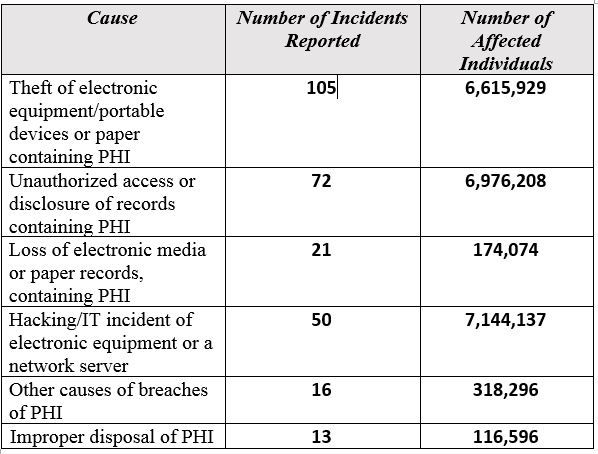
\includegraphics [scale=1]{Data_Breach_table_2013_2014.JPG}
\end{center}

Medical interns is 

 \subsection{Study problem:}
In healthcare sector, there is a rare knowledge about how neutralization techniques are utilized by medical interns in the Saudi's hospitals as they have access privileges to the patient's Electronic Medical Records (EMR). Also, a little is known to which extent neutralization techniques can participate in the violation intention of privacy polices during medical internship period.This empirical study aims at bridging the gap in the literature by considering and evaluating the current security awareness of medical interns in Saudi hospitals and to which extent they adhere to the hospital's policies that are existed to protect patients information privacy. Furthermore, the role of the neutralization techniques on the hospitals' security posture and the ability of these techniques to predict medical interns' intention to violate patient privacy.
\subsection{Theoretical Background:}
\subsubsection{Neutralisation Theory:}
In 1957, Techniques of Neutralization was firstly introduced by \citet{Sykes1957} in criminology field in order to understand juvenile delinquency. According to \cite{Rogers1974}, Neutralization is "a method whereby an individual renders behavioural norms inoperative,thereby freeing himself to engage in behaviour which would otherwise be considered deviant." The theory postulated that offenders employed one or more techniques as defence mechanisms to justify their deviant behaviour prior or after they committed a violence or crime, thereby they convince them self that their deviant behaviour is acceptable regardless of social norm principles \cite{Teh2015}.In their original work, \citet{Sykes1957}have proposed five neutralisation (rationalisation) techniques that juvenile criminals may use to explain their deviant behaviour.  
\begin{itemize}
\item \textbf{The Denial of responsibility:} The centre principle of this technique is that the offender refuse to accept the blame of his/her deviant behaviour and redirect the responsibility of action in question to alternative source.Here, the offender may claim that his/her deviant behaviour had occurred due to accident or lack of control\cite{Sykes1957}.   
\item \textbf{The Denial of Injury:} the offender considers that the result of his/her potential deviant action is harmless, thus, no worry that anyone could get hurt badly if he/she engaging in it\cite{Sykes1957}. 
\item \textbf{The denial of a victim:} the offender claims that the injury resulted from the deviant action is a kind of rightful punishment or retaliation as the victim deserve his/her action consequences\cite{Sykes1957}.   
\item \textbf{The condemnation the condemner:} In this techniques, the offender tend to develop "a rejection of the rejectors" and "shifts the focus of attention from his own deviant acts to the motives and behaviour of those who disapprove of his violations. His condemners, he may claim, are hypocrites, deviants in disguise, or im subtle alchemy the delinquent moves him impelled by personal spite."\cite{Sykes1957}.
\item \textbf{The appeal to higher loyalty:}The offender employed this neutralization technique in order to escape a dilemma that force him/her to choose between confronting with small group interests such as friends, family members, etc or violating a law\cite{Sykes1957}.    
\end{itemize}
Later on, criminology scientists \citet{Rogers1974} and \citet{Minor1981} introduced two techniques as extensions to \citet{Sykes1957} theory, which are:
\begin{itemize}
\item \textbf{Metaphor of the ledger:} the offender argues that his/her previous good acts and rules compliance recompense his/her occasional wrongdoing behaviour\citet{Rogers1974}.
\item \textbf{Defense of necessity:} Here, the offender argues based on the idea that nobody should feel shame or guilt if the situation requires an act that can result breaking rules\cite{Minor1981}.
\end{itemize}

% here talke about employee compliance and it relationship to information privacy violation in healthcare
In the information security context \citet{Siponen2010}conducted an empirical study, and they argue that the employee intention to violation information security policies can be explained by neutralisation factors. The study proposed a theoretical model to test the impact of formal and informal sanctions along with shame on the employee violation intention and the effect of neutralisation factors to rationalise such behaviour. The finding revealed that the organization sanctions alone were not enough to decrease or prevent information policies violation intention as the employees tend to utilise neutralisation techniques to minimise the perceived harm of sanctions. Based on the findings,  authors suggested that the management should consider the importance of neutralisation factors during their efforts to develop and implement information security policies and security awareness champagnes.      

Further empirical study in Malaysia by \citet{Teh2015}, aimed to investigated the organizational factors that influence employees neutralization behavior toward information security polices violations. The study model contains four main  factors include role conflict and role ambiguity from the security literature as well as tow factors drawn form social exchange theory, which were job satisfaction and organizational commitment. A total sample of 246 employees, working in nine Malaysian banks, participated in this study. The results showed that role conflict had a positive influence on employees neutralization techniques toward ISP violation. In contrast , organization commitment, job satisfaction and role ambiguity had insignificant affect on neutralization techniques toward information security policy violation. 

Another empirical study by\citet{Kim2014} proposed an integrative behavioural model based on theory planned behaviour, protraction motivative theory and rational choice theory from social psychology science and neutralization theory from criminology field. The goal was to understand the behavioural factors that affected the employee actions toward compliance with organization information security polices. The authors used survey disseminated to 32 companies within 10 industries and a sample of 194 participants was collected. The results showed that neutralization techniques significantly weaken employee intention toward information security policies compliance. Also, response efficacy and normative beliefs positively impacted employees' intention to comply with the organization's security policies.

\citet{Morris} examined digital piracy as an illegal behaviour via several theories applied in criminology field. Using retrospective(self-reported) and prospective (willingness to engage) models, authors explored the role of Neutralisation techniques when controlling variable from  well-known criminology theories such Self-Control (SC), social learning (SL) and microanomie (strain).They found, using a sample of 585 undergraduate students from two universities, that techniques of neutralisation had a positive and direct effect on students willingness to participate in illegal downloading of music CD over video piracy. Also, from the retrospective model point view, the role of neutralisation had modest effect on music and video piracy over software piracy and can consider as a theoretical predictor for students potential digital piracy. These findings consistent with \cite{Ingram2008} study about the impact of neutralisation techniques on on-line music piracy, who found that those techniques were statistically important to predict students' potential involvement in copying online music. In contrast, \cite{Hinduja2007} found that a weak relationship between online software piracy and the role of neutralization techniques. 
    
\subsection{Research Model and hypotheses:}
Based on previous the scholars result in criminology \cite{Sykes1957}, and information security fields \cite{Siponen2010,Teh2015,Kim2014}. Individuals may intend to preserve peaceful images about themselves by justifying their deviant actions\cite{Kim2014}. In information security field, when an employee breaks an organization policy, he or she may defend his/her non-compliance behavior by providing justification reasons. Thus, Neutralization theory gives a set of rationalized techniques that an employee may use in order to excuse himself/herself and to explain why he/she intend to commit or has committed information security policy violation. In our study, we intend to investigate the role of neutralization techniques to predict the problem of information privacy policies violation and how these techniques affect the intention of medical interns for non-compliance behavior.In this study, we adopt \cite{Siponen2010,Teh2015} approaches by analyzing the neutralization theory as a single second order construct called (Neutralization).The reason is that Neutralization consisted of several first-order sub-constructs (Denial of responsibilities, Denial of injury, defense of necessity, condemnation of the condemners, Appeal of higher loyalties and the Metaphor of ledger) and each of them consider as a distinct dimension with a set of corresponding measurement items work as indicators. Thus, the first order constructs load their results in the second order construct and both can be modeled as reflective. 
Therefore, based on the above deliberation, we have hypothesized the following :\\H1: \textit{Neutralization is directly and positively affects the intention of Medical Interns (MI) to violate the hospital's information privacy polices   \textbf{}} 

\graphicspath{ {image/} }
\begin{center}
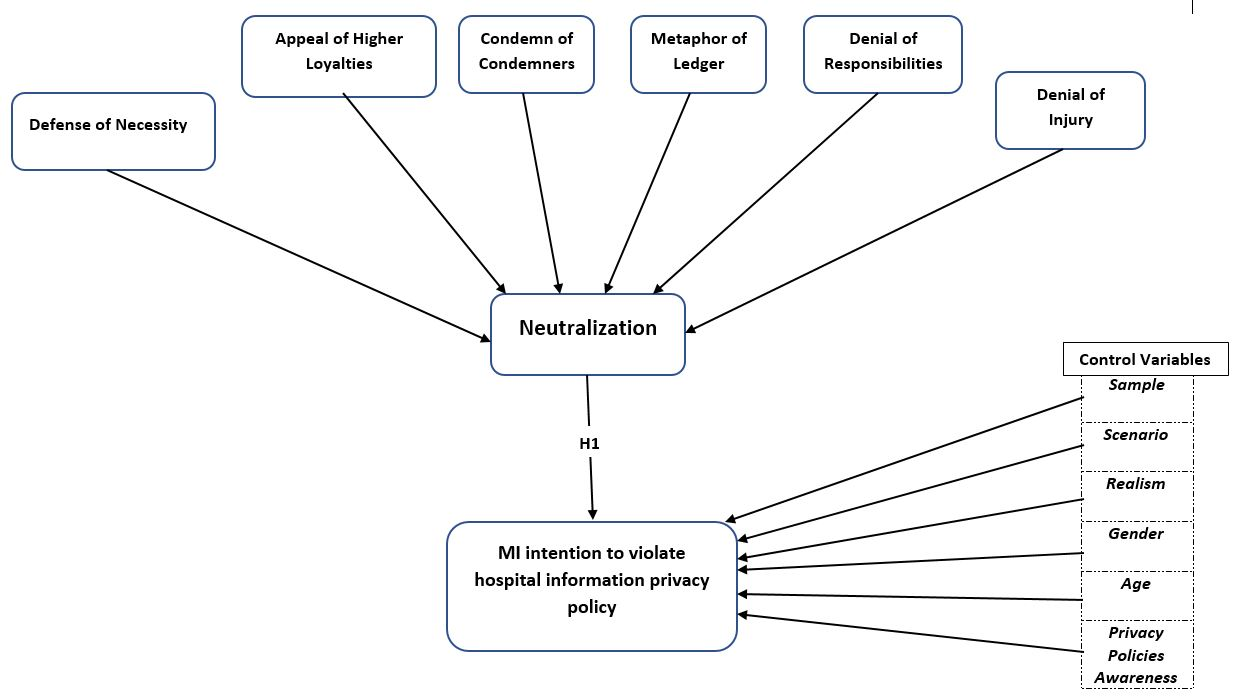
\includegraphics [scale=0.4]{Research_Model_Fv.JPG}
\end{center}
\begin{center}
\title{ Initial Research Model}
\end{center}

\subsubsection{Participants:}
The authors' collected their data from Medical Interns(MI) within Saudi Arabia Hospitals.They reviewed a list of medical colleges within Saudi Universities(See Appendix A) and chose four of them because they have formal security procedures and policies to protect patient information privacy.These universities are King Saud bin Abdulaziz For Health Sciences University, king Saud University, Al-Imam Muhammad Ibn Saud Islamic University and King Abdulaziz University.The first author has a previous experience in Saudi health care sector as an application analyst. This afforded our study the opportunity to access and contact the responsible people of Medical Internship programs in each university to explained purpose of the study. Thereafter, a permission and assistance to disseminate the survey were granted.The Medical interns(MI) were invited to participate in the survey via their official university emails, which included an on line link to the questionnaire. 
\\
\subsubsection{Measures:}
\subparagraph{Construction of variables:} Our study questionnaire constructs and variables were derived from several validated instruments that have been tested and verified in information security context. Also, the majority of the adapted  variables were modified to fit the purpose and context of the study. A complete list of constructs and variables is summarized in (Appendix B).

\subparagraph{Neutralization Techniques:} Based on \cite{Siponen2010} recommendations, we tailor measurements for each of the neutralization techniques to match our study objectives. This survey included 18 adapted items indicate six techniques "the defense of necessity, denial of injury, metaphor of Ledger, condemnation of condemners, denial of responsibility and appeal to higher loyalties ". The respondents were asked to revealed their level of agreement based on seven points Likert scale (e.g, 1=Strongly disagree; 7=strongly agree). \\
\cite{Siponen2010} reported that scenario method is an appropriate approach to assess deviant/ abuse behavior intention. According to \citet{trevino1992experimental} , a scenario is a vignettes that "\textit{present subjects with written descriptions of realistic situations and then request responses on a number of rating scales that measure the dependent variables of interest} ". Thereby, to measure the dependent variable, Intention to violate hospital Information Privacy Policy, we followed \cite{Siponen2010,Teh2015} research by using a single item that  directly came after the scenario (Appendix B).In this study, four scenarios covered several security area were developed, and two of them were nominated based on the recommendations from three of the MI program managers and four medical interns.\\
Once the respondents completed reading each scenario, they were asked to rate the likelihood to imitate a particular violation act that one of the scenario characters did. The response scale was base on seven points Likert scale(e.g 1=Very Unlikely,...., 7=Very Likely). Thereafter, a single item was presented to measure the degree of scenario realism. 
\subparagraph {Control variables: } include age, gender, work experience, level of privacy policies awareness, and realism.
 

\section{Plan and Future Work:}
This section illustrates my following steps in my PhD theses. The results from the first year experiment will be the foundation to understand the current level of medical interns' overall security awareness about privacy polices as well as the potential role of neutralization techniques in the intention to breach patient privacy.Thereafter, based on the results, I will extend my current work by examining the antecedents factors of neutralization techniques in health care context. Also,I Intend to have an access to security  polices and security incident reports from one or more Saudi hospitals in order to understand and analyze the current state of security design for the favor of medical interns. My aim in the second year is to determine security policies deficiencies and preform privacy polices and security incidents analysis. By doing that I can get a deeper insight in the security level and develop a formal approach to develop better privacy polices for the hospitals and enhance privacy awareness program designed for the healthcare members, specifically medical interns. Also, I will finalize my first year study in order make it ready for publishing. To summarize my future plan:
\begin{itemize}
	\item Determining the organizational factors that can reduce the affect of Neutralization techniques in order to increase privacy protection.  
	 \item Evaluating current security state in Saudi hospitals by gather and analyze hospital's information polices that designed to protect patient privacy there.
	 \item Developing a framework for hospitals that aim to enhance both patient information privacy policies and privacy awareness programs by considering the role of Neutralization techniques.
\end{itemize}
  
\section{Activities in First Year:}

\begin{itemize}
	\item I have attend two days workshop for qualitative analysis using Nvivo tool at Glasgow caledonian university University.
	\item I have attend "Internet of Things meets Cyber security" conference in Edinburgh April 20,2017
	\item I have attend first Ad workshop.
\end{itemize}

\section{First Year Summary:}
% Bibliography
\addcontentsline{toc}{chapter}{Bibliography}
\bibliographystyle{IEEEtran}

\bibliography{bibliography/dissertation}

\end{document}
